\documentclass[11pt,a4paper]{article}

% ─── packages ────────────────────────────────────────────────────────────────
\usepackage[margin=2.4cm]{geometry}
\usepackage[T1]{fontenc}
\usepackage{lmodern}
\usepackage{amssymb}
\usepackage{xcolor}
\usepackage{colortbl}
\usepackage{titlesec}
\usepackage{enumitem}
\usepackage{booktabs}
\usepackage{array}
\usepackage{tabularx}
\usepackage{fancyhdr}
\usepackage{tikz}
\usepackage{pgfgantt}
\usepackage{hyperref}
\usetikzlibrary{arrows.meta,positioning}

% ─── colours (restrained / formal) ───────────────────────────────────────────
\definecolor{primary}{HTML}{1B3B5F}   % navy
\definecolor{steel}{HTML}{4A6E8A}     % muted steel blue
\definecolor{rule}{HTML}{1B3B5F}
\definecolor{rowgray}{HTML}{F0F3F6}

\hypersetup{colorlinks=true, linkcolor=primary, urlcolor=primary}

% ─── headings ────────────────────────────────────────────────────────────────
\titleformat{\section}{\large\bfseries\color{primary}}{\thesection.}{0.5em}{}
\titleformat{\subsection}{\normalsize\bfseries\color{primary}}{\thesubsection}{0.5em}{}
\titlespacing*{\section}{0pt}{1.0em}{0.45em}
\titlespacing*{\subsection}{0pt}{0.7em}{0.3em}

% ─── header / footer ─────────────────────────────────────────────────────────
\pagestyle{fancy}
\fancyhf{}
\renewcommand{\headrulewidth}{0.4pt}
\fancyhead[L]{\small\color{primary}Street View Robot --- Project Work Plan}
\fancyhead[R]{\small\color{primary}Group 9}
\fancyfoot[C]{\small\color{gray}\thepage}

\setlist[enumerate]{leftmargin=1.6em,topsep=2pt,itemsep=1.5pt}
\setlist[itemize]{leftmargin=1.4em,topsep=2pt,itemsep=1.5pt}
\renewcommand{\arraystretch}{1.25}

% ═══════════════════════════════════════════════════════════════════════════════
\begin{document}

% ─── title block ─────────────────────────────────────────────────────────────
\begin{center}
{\color{primary}\rule{\linewidth}{1.2pt}}\\[6pt]
{\LARGE\bfseries\color{primary} Project Work Plan}\\[5pt]
{\Large Street View Robot}\\[3pt]
{\normalsize\itshape A mobile robot for 360\textdegree{} point-cloud reconstruction of indoor spaces}\\[6pt]
{\color{primary}\rule{\linewidth}{1.2pt}}
\end{center}

\vspace{2pt}
\begin{center}
\begin{tabular}{rl@{\hspace{2.2cm}}rl}
\textbf{Project:} & Street View Robot & \textbf{Supervisor:} & Mr.\ Rajaei Khatib\\
\textbf{Team:} & Group 9 (5 members) & \textbf{Date:} & 31 May 2026\\
\textbf{Platform:} & Raspbot V2 / Raspberry Pi 5 & \textbf{Duration:} & 5 working days\\
\end{tabular}
\end{center}
\vspace{4pt}

% ─── 1. introduction ─────────────────────────────────────────────────────────
\section{Introduction}
This document presents the work plan for the \textit{Street View Robot} project. The objective of
the project is to design and implement a mobile robot capable of autonomously traversing an indoor
environment and constructing a three-dimensional point-cloud representation of its surroundings at
each sampled location. Individual scans are subsequently merged into a single, room-scale
360\textdegree{} reconstruction.

The robot is built on the Raspbot V2 platform---a Raspberry Pi~5 chassis with four Mecanum wheels
providing omnidirectional motion through an I\textsuperscript{2}C motor driver. Depth sensing is
provided by an Intel RealSense D405, a factory-calibrated stereo infrared camera. Additional onboard
sensors (an ultrasonic rangefinder and four infrared line-tracking sensors) support obstacle
detection and autonomous line following. The complete system is exposed through a Python hardware
abstraction layer and supports two modes of navigation: manual keyboard control and autonomous line
following.

% ─── 2. aim and objectives ───────────────────────────────────────────────────
\section{Aim and Objectives}
\textbf{Aim.} To deliver a functional mobile-robot system that incrementally builds a 360\textdegree{}
point-cloud map of a room through coordinated navigation and stereo depth perception.

\noindent\textbf{Objectives.}
\begin{enumerate}
\item Assemble the robot chassis and configure the Raspberry Pi software environment.
\item Implement a hardware abstraction layer for movement, sensing, and image capture.
\item Compute depth from the stereo infrared pair and generate 3D point clouds.
\item Register and merge multiple views into a single 360\textdegree{} point cloud per location.
\item Implement the two navigation modes (manual control and autonomous line following).
\item Design and 3D-print a rigid mounting bracket for the depth camera.
\item Integrate, test, and document the complete system.
\end{enumerate}

% ─── 3. scope and deliverables ───────────────────────────────────────────────
\section{Scope and Deliverables}
The project will deliver the following:
\begin{itemize}
\item An assembled, operational robot with the depth camera mounted on a custom 3D-printed bracket.
\item A Python API abstracting all hardware into method calls (e.g. \texttt{forward()}, \texttt{capture\_stereo()}, \texttt{set\_tilt()}).
\item A perception pipeline that produces a 360\textdegree{} point cloud at each sampled location and merges locations into a room-scale scan.
\item Two functional navigation modes: manual (keyboard) and autonomous (line following).
\item Source code, technical documentation, and a final demonstration.
\end{itemize}

% ─── 4. methodology ──────────────────────────────────────────────────────────
\section{Methodology}
The technical approach is organised around the data-processing pipeline shown below.

\begin{center}
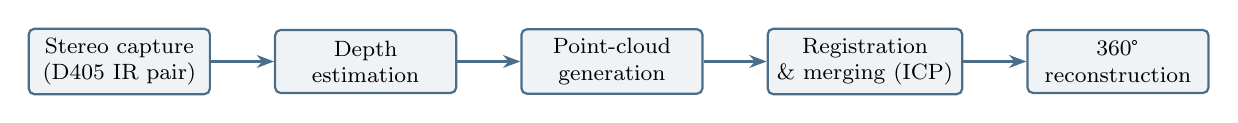
\begin{tikzpicture}[
  node distance=8mm, font=\footnotesize,
  box/.style={draw=steel,fill=rowgray,rounded corners=2pt,minimum height=8mm,minimum width=23mm,align=center,thick},
  ar/.style={-{Stealth[length=2.2mm]},steel,thick}
]
\node[box] (a) {Stereo capture\\(D405 IR pair)};
\node[box,right=of a] (b) {Depth\\estimation};
\node[box,right=of b] (c) {Point-cloud\\generation};
\node[box,right=of c] (d) {Registration\\\& merging (ICP)};
\node[box,right=of d] (e) {360\textdegree{}\\reconstruction};
\draw[ar](a)--(b);\draw[ar](b)--(c);\draw[ar](c)--(d);\draw[ar](d)--(e);
\end{tikzpicture}
\end{center}

\subsection{Depth Estimation}
Depth is computed from the rectified left/right infrared images using block-matching (semi-global
block matching). Disparity is converted to metric depth using the camera's factory-calibrated focal
length and stereo baseline ($Z = f_x \cdot b / d$). The result is validated against the camera's
built-in depth stream.

\subsection{Point-Cloud Generation}
Each depth image is back-projected into 3D space using the pinhole camera model and the factory
intrinsics, producing one point cloud per viewpoint.

\subsection{Registration and Merging}
At each location the robot rotates through a sequence of known angular steps, capturing a point cloud
at each step. Clouds are aligned using the Iterative Closest Point (ICP) algorithm, initialised with
the robot's known rotation, and combined into a single 360\textdegree{} point cloud. Outlier removal
and voxel down-sampling are applied to control noise and density.

\subsection{Navigation and Control}
Omnidirectional motion is achieved through Mecanum-wheel kinematics issued over I\textsuperscript{2}C.
In manual mode the robot is driven via keyboard input; in autonomous mode it follows a taped path
using its four infrared sensors and halts at cross-shaped stop markers to trigger the capture routine.

\subsection{Camera Mounting}
A rigid bracket will be designed and 3D-printed to fix the D405 ($42 \times 42 \times 23$\,mm, 58\,g,
secured by two M3 screws) to the chassis at a fixed, level, and repeatable pose---a prerequisite for
accurate point-cloud registration.

% ─── 5. work plan & schedule ─────────────────────────────────────────────────
\section{Work Plan and Schedule}
The project is scheduled across five working days. Development and implementation are to be completed
by the \textbf{middle of Day~4}; the remaining time is allocated to integration, testing, and
preparation of the final demonstration.

\subsection{Work Breakdown}
\begin{center}
\small
\begin{tabularx}{\linewidth}{@{}p{0.7cm}p{3.4cm}Xp{1.6cm}@{}}
\toprule
\textbf{ID} & \textbf{Phase} & \textbf{Tasks} & \textbf{Duration}\\
\midrule
\rowcolor{rowgray} 1 & Setup \& Integration & Chassis assembly; Raspberry Pi OS, I\textsuperscript{2}C and camera configuration; software environment; network access. & Day 1\\
2 & Perception Core & Stereo depth estimation; point-cloud generation; validation against factory depth. & Day 1--2\\
\rowcolor{rowgray} 3 & Mobility \& API & Hardware API; Mecanum motion; servo and sensor control; manual navigation mode. & Day 2--3\\
4 & 360\textdegree{} Reconstruction & Rotate--capture--merge routine; ICP registration; single-location 360\textdegree{} cloud. & Day 3\\
\rowcolor{rowgray} 5 & Autonomous Navigation & Line-following control; stop-marker detection; capture-routine integration. & Day 3--4\\
6 & Mechanical & Camera-mount measurement, design, 3D printing and fitting. & Day 1--3\\
\rowcolor{rowgray} 7 & Integration \& Testing & Multi-location collection; system testing; refinement. & Day 4\\
8 & Documentation \& Demo & Final documentation; demonstration preparation. & Day 4--5\\
\bottomrule
\end{tabularx}
\end{center}

\subsection{Schedule (Gantt Chart)}
\begin{center}
\begin{ganttchart}[
  hgrid, vgrid={*1{draw=gray!18}},
  x unit=1.18cm, y unit title=0.6cm, y unit chart=0.5cm,
  canvas/.append style={draw=gray!40},
  title/.append style={fill=primary,draw=primary},
  title label font=\small\bfseries\color{white},
  bar/.append style={fill=steel,draw=primary,rounded corners=1pt},
  bar height=0.55, bar label font=\footnotesize,
  milestone/.append style={fill=primary,draw=primary},
  milestone label font=\footnotesize\bfseries,
]{1}{10}
\gantttitle{Day 1}{2}\gantttitle{Day 2}{2}\gantttitle{Day 3}{2}\gantttitle{Day 4}{2}\gantttitle{Day 5}{2}\\
\ganttbar{Setup \& integration}{1}{2}\\
\ganttbar{Perception core}{1}{4}\\
\ganttbar{Mobility \& API}{3}{5}\\
\ganttbar{360\textdegree{} reconstruction}{5}{6}\\
\ganttbar{Autonomous navigation}{5}{7}\\
\ganttbar{Camera mount (3D print)}{1}{6}\\
\ganttbar{Integration \& testing}{7}{8}\\
\ganttbar{Documentation \& demo}{8}{10}\\
\ganttmilestone{Development complete}{7}\\
\ganttmilestone{Final demonstration}{10}
\end{ganttchart}
\end{center}
\vspace{-2pt}
{\footnotesize\itshape Each day comprises two half-day units. Development is completed at the middle of Day~4 (``Development complete'' milestone).}

% ─── 6. milestones ───────────────────────────────────────────────────────────
\section{Milestones}
\begin{center}
\small
\begin{tabularx}{\linewidth}{@{}p{1.2cm}Xp{2.0cm}@{}}
\toprule
\textbf{No.} & \textbf{Milestone} & \textbf{Target}\\
\midrule
M1 & Robot assembled, Pi configured, camera capturing frames & End of Day 1\\
\rowcolor{rowgray} M2 & Depth estimation and point-cloud generation operational; manual driving working & End of Day 2\\
M3 & 360\textdegree{} point cloud produced at a single location; camera mount fitted & End of Day 3\\
\rowcolor{rowgray} M4 & Both navigation modes integrated; development complete & Mid Day 4\\
M5 & System tested, documented, and demonstrated & End of Day 5\\
\bottomrule
\end{tabularx}
\end{center}

% ─── 7. resources ────────────────────────────────────────────────────────────
\section{Resources and Tools}
\begin{itemize}
\item \textbf{Hardware:} Raspbot V2 chassis, Raspberry Pi 5, Intel RealSense D405, ultrasonic and infrared sensors, 3D printer.
\item \textbf{Software:} Python 3, OpenCV, NumPy, pyrealsense2, Open3D; Raspberry Pi OS (64-bit); CAD/slicing software for the mount.
\end{itemize}

% ─── 8. risk assessment ──────────────────────────────────────────────────────
\section{Risk Assessment}
\begin{center}
\small
\begin{tabularx}{\linewidth}{@{}p{4.3cm}p{1.7cm}X@{}}
\toprule
\textbf{Risk} & \textbf{Impact} & \textbf{Mitigation}\\
\midrule
\rowcolor{rowgray} RealSense driver build fails on Raspberry Pi & High & Allow buffer time on Day 1; develop perception on a laptop in parallel.\\
Poor depth on low-texture surfaces (passive stereo) & Medium & Use textured, well-lit capture environments; tune matching parameters.\\
\rowcolor{rowgray} Inaccurate cloud registration / merging & Medium & Use small rotation steps with high overlap; initialise ICP with the known rotation.\\
3D-print failure or delay & Medium & Begin design on Day 1; prepare a temporary mounting fallback.\\
\rowcolor{rowgray} Network access to the robot unavailable & Low & Use an alternative local network (mobile hotspot) for SSH access.\\
Schedule overrun & Medium & Prioritise manual mode (essential); treat autonomous mode as secondary; enforce the Day-4 development freeze.\\
\bottomrule
\end{tabularx}
\end{center}

% ─── 9. expected outcomes ────────────────────────────────────────────────────
\section{Expected Outcomes}
On completion, the project is expected to deliver a fully operational robot that navigates an indoor
space, autonomously captures and reconstructs 360\textdegree{} point clouds at multiple locations, and
merges them into a coherent room-scale map. Both navigation modes will be demonstrated, and the depth
camera will be mounted on a purpose-built 3D-printed bracket. All source code and documentation will
be delivered, accompanied by a final demonstration to the supervisor.

\end{document}
